% ============================================================
% Project : THE PHILOSOPHY OF VIABILITY
% Book    : Book I — Ontology of Viability
% Book ID : VS.B01
% Part    : Part I — Identity and Manifestation
% Chapter : Chapter 08 — Comparative Philosophical Examination
% Chapter ID: VS.B01.P01.C08
% File    : 01_method_and_criteria_of_comparison.tex
% Section : Section 01 — Method and Criteria of Comparison
% Section ID: VS.B01.P01.C08.S01
%
% Purpose:
% Establish the methodological commitments, criteria, and
% dialectical procedure governing the comparative examination
% of philosophical traditions in Chapter 08.
%
% Status:
% Complete section draft. Paragraph identifiers are recorded
% in comments and paired with standard hyperref labels.
% ============================================================

\section{Method and Criteria of Comparison}
\label{sec:ch08-method-and-criteria}

\subsection{The Object and Scope of Comparison}
\label{sec:ch08-s01-ss01}

% Structural ID: VS.B01.P01.C08.S01.SS01.P001
\phantomsection\label{para:VS.B01.P01.C08.S01.SS01.P001}
The comparative examination undertaken in this chapter concerns
the ontological problems developed in Part I: Being and Identity,
their analytical distinction and ontological inseparability,
Determination, Invariance, Unity, Plurality, Expression,
Manifestation, Persistence, and Continuity. Its purpose is not
to collect historical statements that resemble the terminology
of the Philosophy of Viability. It is to examine whether, and
under what conditions, different philosophical accounts address
the same problems, rely on comparable assumptions, reach
compatible conclusions, or remain separated by irreducible
differences.

% Structural ID: VS.B01.P01.C08.S01.SS01.P002
\phantomsection\label{para:VS.B01.P01.C08.S01.SS01.P002}
The object of comparison is therefore not a word considered in
isolation, nor a doctrine detached from the questions that give
it meaning. It is a philosophically situated account: a set of
claims, distinctions, arguments, explanatory commitments, and
limitations concerning a specified ontological problem. A term
such as ``being,'' ``substance,'' ``essence,'' ``identity,''
``unity,'' or ``change'' cannot be treated as a stable common
unit merely because it appears in more than one tradition.
Its function must be reconstructed within the argument in which
it occurs.

% Structural ID: VS.B01.P01.C08.S01.SS01.P003
\phantomsection\label{para:VS.B01.P01.C08.S01.SS01.P003}
The comparison is also limited by the scope of Part I. It
examines the conceptual and ontological foundations already
developed there; it does not attempt to settle in advance the
architecture of the four proposed fundamental realms and three
intermediate hubs, the ontological status of Light, or the
dynamics of Being. Those questions belong to their respective
investigations. They may become relevant when a historical
position bears directly upon them, but their later treatment
must not be anticipated or treated as already established.

% Structural ID: VS.B01.P01.C08.S01.SS01.P004
\phantomsection\label{para:VS.B01.P01.C08.S01.SS01.P004}
The chapter does not assume that every philosopher examined
offers a complete ontology, or that every tradition organizes
its questions according to the distinctions adopted in this
book. Some accounts address the identity of persons; others
investigate substance, being, essence, change, dependence,
emptiness, non-duality, or the relation between the one and the
many. Their relevance must be established through the problem
they actually investigate, not through an artificial expansion
of their claims into a general theory of identity.

\subsection{Comparative Philosophy and Historical Reconstruction}
\label{sec:ch08-s01-ss02}

% Structural ID: VS.B01.P01.C08.S01.SS02.P001
\phantomsection\label{para:VS.B01.P01.C08.S01.SS02.P001}
A philosophical comparison requires historical reconstruction
before critical evaluation. The position under examination must
first be presented in terms that are faithful to its texts,
conceptual vocabulary, argumentative context, and relevant
historical setting. This requirement is not an instruction to
accept the philosopher's conclusions. It is a condition for
criticizing the position that the philosopher actually
maintained rather than a simplified substitute constructed for
the convenience of the present argument.

% Structural ID: VS.B01.P01.C08.S01.SS02.P002
\phantomsection\label{para:VS.B01.P01.C08.S01.SS02.P002}
Historical reconstruction must distinguish at least four
levels: the philosopher's explicit statements; conclusions
that follow from the philosopher's arguments; interpretations
advanced by later commentators; and reconstructions proposed
for the purposes of the present comparison. These levels may
support one another, but they are not interchangeable. A
commentator's interpretation must not be attributed directly
to the historical thinker without qualification, and an
inference made by the present author must not be presented as
though it were an explicit historical doctrine.

% Structural ID: VS.B01.P01.C08.S01.SS02.P003
\phantomsection\label{para:VS.B01.P01.C08.S01.SS02.P003}
Primary texts have priority when the question concerns what a
philosopher argued, defined, denied, or left unresolved.
Secondary scholarship is indispensable where it clarifies
historical context, textual transmission, disputed readings,
technical vocabulary, or interpretive disagreement. It may
also identify difficulties that are not immediately visible
in a translated passage. Nevertheless, secondary scholarship
cannot silently replace the primary text as the basis for
attributing a position.

% Structural ID: VS.B01.P01.C08.S01.SS02.P004
\phantomsection\label{para:VS.B01.P01.C08.S01.SS02.P004}
The textual history of a work must also be taken into account.
A philosophical corpus may contain works of different dates,
layers of composition, disputed authorship, editorial
arrangement, or translation histories. Where such matters
affect the interpretation, the comparison must state the
relevant qualification. It must not construct a single,
uniform doctrine from texts whose relation to one another
remains historically or philosophically disputed.

% Structural ID: VS.B01.P01.C08.S01.SS02.P005
\phantomsection\label{para:VS.B01.P01.C08.S01.SS02.P005}
Translation requires particular care. A translated term may
have several possible equivalents, while one word in the
receiving language may conceal distinctions present in the
original. The comparison must therefore avoid treating
translated vocabulary as proof of conceptual identity. Where
a technical term is decisive, its original form, range of
meaning, and role in the argument should be identified to the
extent that the available textual evidence permits.

\subsection{Shared Questions Without Presupposed Equivalence}
\label{sec:ch08-s01-ss03}

% Structural ID: VS.B01.P01.C08.S01.SS03.P001
\phantomsection\label{para:VS.B01.P01.C08.S01.SS03.P001}
A meaningful comparison requires a shared question, but a
shared question does not require identical concepts. Two
philosophers may investigate how something remains what it is
through change while offering fundamentally different
accounts of what the relevant ``something'' is, what counts
as change, and what kind of continuity requires explanation.
Their positions can be compared because the problem is
sufficiently related, even though their conceptual solutions
are not equivalent.

% Structural ID: VS.B01.P01.C08.S01.SS03.P002
\phantomsection\label{para:VS.B01.P01.C08.S01.SS03.P002}
The comparative procedure must consequently distinguish
between a common problem, a common term, a common conceptual
function, and a common conclusion. These are different forms
of relation. A common problem may exist without a common
term; a common term may conceal different functions; similar
functions may depend on different assumptions; and similar
conclusions may be reached through incompatible arguments.
No one of these relations establishes the others.

% Structural ID: VS.B01.P01.C08.S01.SS03.P003
\phantomsection\label{para:VS.B01.P01.C08.S01.SS03.P003}
For this reason, the concepts developed in Part I must not be
imposed retrospectively upon historical thinkers. A
philosopher's account of substance must not automatically be
translated into an account of Identity. An account of unity
must not automatically be treated as a theory of the unity of
identity. A theory of what remains unchanged must not
automatically be classified as a theory of Invariance in the
specific sense examined in this book. Each proposed
correspondence requires an argument that identifies both
what is shared and what remains different.

% Structural ID: VS.B01.P01.C08.S01.SS03.P004
\phantomsection\label{para:VS.B01.P01.C08.S01.SS03.P004}
The same caution applies in the opposite direction. The
historical philosopher's conceptual framework must not be
used to redefine the terms of the Philosophy of Viability
without examination. The comparison is not a translation
exercise in which one system supplies the vocabulary and the
other supplies examples. It is an encounter between
conceptual frameworks whose points of contact and
incompatibility must themselves become objects of analysis.

% Structural ID: VS.B01.P01.C08.S01.SS03.P005
\phantomsection\label{para:VS.B01.P01.C08.S01.SS03.P005}
A comparison is therefore strongest when it makes the
translation problem explicit. It should state which term or
distinction is being compared, why the comparison is
justified, what conceptual loss may result from translation,
and which aspects of the original account cannot be
adequately represented through the vocabulary of the other
system. Where no sufficiently defensible correspondence can
be established, the correct result is not forced equivalence
but a clearly stated limit of comparison.

\subsection{The Dialectical Procedure}
\label{sec:ch08-s01-ss04}

% Structural ID: VS.B01.P01.C08.S01.SS04.P001
\phantomsection\label{para:VS.B01.P01.C08.S01.SS04.P001}
The examination follows a symmetrical dialectical procedure.
Symmetry here does not mean that the two positions must be
equally correct, equally comprehensive, or equally supported.
It means that each must be examined under comparable
standards of interpretive fairness and argumentative
seriousness. The Philosophy of Viability must not be exempted
from criticism merely because it supplies the framework of
the present book, and a historical position must not be
weakened merely because it is being examined from the
standpoint of a different ontology.

% Structural ID: VS.B01.P01.C08.S01.SS04.P002
\phantomsection\label{para:VS.B01.P01.C08.S01.SS04.P002}
The procedure begins by reconstructing the philosopher's
relevant position from primary sources and historically
responsible scholarship. It then identifies the precise
ontological question at issue and formulates the philosopher's
answer in its strongest defensible form. Only after this
reconstruction may the comparison identify the assumptions
on which the position depends and the consequences that
follow from it.

% Structural ID: VS.B01.P01.C08.S01.SS04.P003
\phantomsection\label{para:VS.B01.P01.C08.S01.SS04.P003}
The next movement asks what the reconstructed position
challenges in the Philosophy of Viability. The objection
must be formulated as a serious philosophical difficulty,
not as a rhetorical summary or an objection that can be
dismissed by repeating a distinction already asserted in
Part I. It should identify the premise, inference, conceptual
separation, or explanatory commitment that the historical
position places under pressure.

% Structural ID: VS.B01.P01.C08.S01.SS04.P004
\phantomsection\label{para:VS.B01.P01.C08.S01.SS04.P004}
The response must then be developed from arguments and
commitments actually established in Part I. If the response
requires a premise that has not been established, that
premise must be identified as a proposal, a provisional
construction, or an open problem. The response must not
silently strengthen the ontology merely to defeat an
objection. Nor may it use later topics as though their
arguments had already been completed.

% Structural ID: VS.B01.P01.C08.S01.SS04.P005
\phantomsection\label{para:VS.B01.P01.C08.S01.SS04.P005}
The examination next formulates the strongest objection
that the Philosophy of Viability raises against the
historical position. This objection must address the
position's actual commitments and explanatory consequences.
It must not rely on a concept that the historical philosopher
does not recognize without first explaining how that concept
can be applied to the position without distorting it.

% Structural ID: VS.B01.P01.C08.S01.SS04.P006
\phantomsection\label{para:VS.B01.P01.C08.S01.SS04.P006}
A fair comparison then reconstructs the strongest available
defence of the historical philosopher. This stage is
essential because an objection may reveal a limitation in
the present reconstruction rather than a defect in the
historical position. The defence may require a distinction,
qualification, or interpretive possibility that the initial
presentation did not adequately recognize. Where it does,
the earlier reconstruction must be revised before a final
assessment is attempted.

% Structural ID: VS.B01.P01.C08.S01.SS04.P007
\phantomsection\label{para:VS.B01.P01.C08.S01.SS04.P007}
The procedure may continue through further objections and
responses where the dispute requires them. It does not
prescribe a fixed number of argumentative exchanges. Its
completion is determined by the point at which the relevant
positions, principal assumptions, strongest objections,
available responses, and remaining uncertainties have been
made sufficiently explicit for a responsible assessment.

% Structural ID: VS.B01.P01.C08.S01.SS04.P008
\phantomsection\label{para:VS.B01.P01.C08.S01.SS04.P008}
The final assessment identifies the points of convergence,
the decisive differences, the limits of each position, and
the questions that remain unresolved. It must also state
whether the comparison provides a reason to retain, qualify,
revise, or suspend any claim in the Philosophy of Viability.
A historical position may expose a weakness without
supplying a complete alternative; conversely, the present
ontology may identify a difficulty in a historical account
without thereby resolving the entire problem.

% Structural ID: VS.B01.P01.C08.S01.SS04.P009
\phantomsection\label{para:VS.B01.P01.C08.S01.SS04.P009}
The dialectical movement is therefore iterative rather than
a one-directional sequence ending automatically in the
victory of one framework. Reconstruction can correct the
formulation of an objection; a defence can require revision
of the initial interpretation; a response can reveal an
unproved premise; and the final assessment can leave a
question open. The procedure is designed to make such
revisions visible rather than to conceal them.

\begin{center}

% ============================================================
% Project : THE PHILOSOPHY OF VIABILITY
% Book    : Book I — Ontology of Viability
% Book ID : VS.B01
% Chapter : 08 — Comparative Philosophical Examination
% Section : 01 — Method and Criteria of Comparison
% Asset ID: VS.B01.P01.C08.S01.SS04.P009.DG01
% Type    : DG — Diagram
% File    : dialectical_comparison_cycle.tex
% Purpose : Represent the iterative and revisable structure
%           of the comparative dialectical procedure.
% ============================================================

\begin{figure}[htbp]
\centering

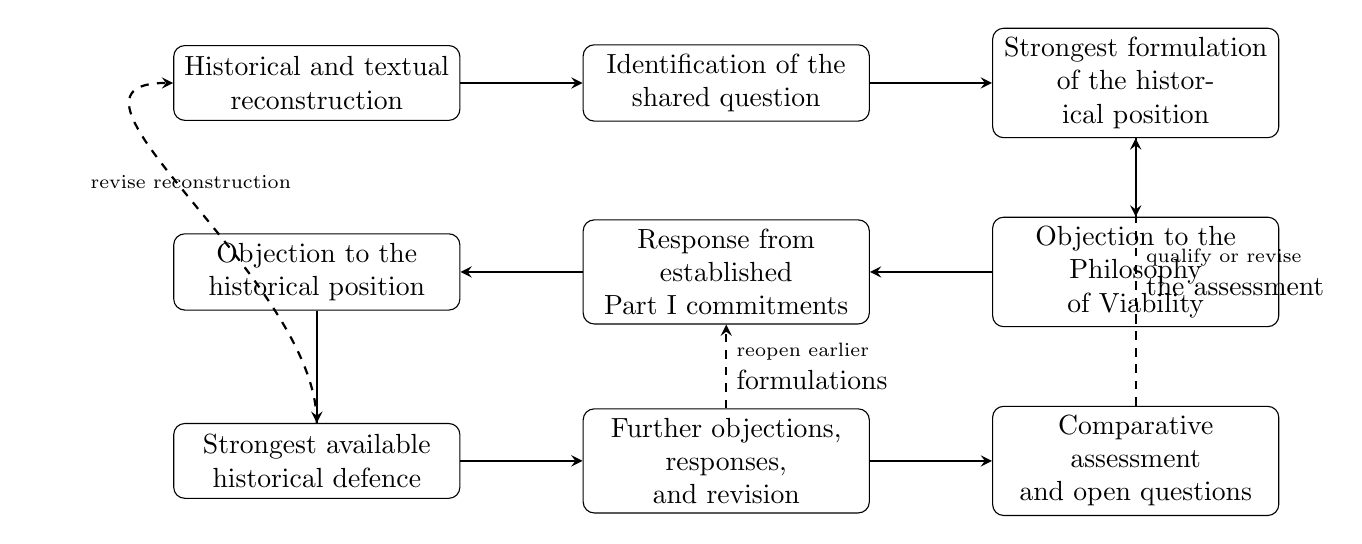
\begin{tikzpicture}[>=stealth]

% Nodes
\node[draw, rounded corners, align=center,
      text width=3.4cm, minimum height=0.95cm]
      (A) at (0,0)
      {Historical and textual\\reconstruction};

\node[draw, rounded corners, align=center,
      text width=3.4cm, minimum height=0.95cm]
      (B) at (5.2,0)
      {Identification of the\\shared question};

\node[draw, rounded corners, align=center,
      text width=3.4cm, minimum height=0.95cm]
      (C) at (10.4,0)
      {Strongest formulation\\of the historical position};

\node[draw, rounded corners, align=center,
      text width=3.4cm, minimum height=0.95cm]
      (D) at (10.4,-2.4)
      {Objection to the\\Philosophy of Viability};

\node[draw, rounded corners, align=center,
      text width=3.4cm, minimum height=0.95cm]
      (E) at (5.2,-2.4)
      {Response from established\\Part I commitments};

\node[draw, rounded corners, align=center,
      text width=3.4cm, minimum height=0.95cm]
      (F) at (0,-2.4)
      {Objection to the\\historical position};

\node[draw, rounded corners, align=center,
      text width=3.4cm, minimum height=0.95cm]
      (G) at (0,-4.8)
      {Strongest available\\historical defence};

\node[draw, rounded corners, align=center,
      text width=3.4cm, minimum height=0.95cm]
      (H) at (5.2,-4.8)
      {Further objections,\\responses, and revision};

\node[draw, rounded corners, align=center,
      text width=3.4cm, minimum height=0.95cm]
      (I) at (10.4,-4.8)
      {Comparative assessment\\and open questions};

% Main argumentative movement
\draw[->, thick] (A) -- (B);
\draw[->, thick] (B) -- (C);
\draw[->, thick] (C) -- (D);
\draw[->, thick] (D) -- (E);
\draw[->, thick] (E) -- (F);
\draw[->, thick] (F) -- (G);
\draw[->, thick] (G) -- (H);
\draw[->, thick] (H) -- (I);

% Revision and feedback relations
\draw[->, dashed, thick]
  (G.north) to[out=90,in=180]
  node[above, align=center]
  {\scriptsize revise reconstruction}
  (A.west);

\draw[->, dashed, thick]
  (H.north) to[out=90,in=270]
  node[right, align=left]
  {\scriptsize reopen earlier\\formulations}
  (E.south);

\draw[->, dashed, thick]
  (I.north) to[out=90,in=270]
  node[right, align=left]
  {\scriptsize qualify or revise\\the assessment}
  (C.south);

\end{tikzpicture}

\caption{The iterative dialectical procedure of comparative examination. The arrows represent the principal argumentative sequence and the dashed arrows represent possible revision and feedback. The diagram does not imply that every comparison must terminate in a final resolution.}
\label{fig:ch08-dialectical-comparison-cycle}

\end{figure}

% ============================================================
% END OF ASSET
% ============================================================

\end{center}

\subsection{Criteria for Evaluating an Ontological Position}
\label{sec:ch08-s01-ss05}

% Structural ID: VS.B01.P01.C08.S01.SS05.P001
\phantomsection\label{para:VS.B01.P01.C08.S01.SS05.P001}
The evaluation of a philosophical position requires more
than a statement of agreement or disagreement. It must
identify the standards under which the position is being
examined and explain why those standards are relevant to
the problem. The criteria below are not a numerical
scoring system, nor do they establish a single hierarchy
of philosophical importance. They provide distinct
questions through which the explanatory and argumentative
performance of a position can be examined.

% Structural ID: VS.B01.P01.C08.S01.SS05.P002
\phantomsection\label{para:VS.B01.P01.C08.S01.SS05.P002}
First, conceptual precision concerns whether the position
distinguishes the concepts on which its argument depends.
A theory may appear to solve a problem because it uses one
term for several different functions. The comparison must
determine whether those functions are genuinely identical,
related but distinct, or insufficiently differentiated.
Conceptual precision is not achieved by multiplying
distinctions without reason; each distinction must perform
an identifiable role in the argument.

% Structural ID: VS.B01.P01.C08.S01.SS05.P003
\phantomsection\label{para:VS.B01.P01.C08.S01.SS05.P003}
Second, ontological adequacy concerns whether the account
addresses the kind of reality its claims purport to explain.
An account of how something is described, recognized, or
represented does not by itself establish an account of
what exists or how it is constituted. In this book,
ontological claims must not be made dependent upon
cognition, language, perception, or self-awareness unless
a separate argument establishes the relevance of such
dependence. The comparison must preserve the distinction
between an ontological account and an epistemological
account.

% Structural ID: VS.B01.P01.C08.S01.SS05.P004
\phantomsection\label{para:VS.B01.P01.C08.S01.SS05.P004}
Third, argumentative validity concerns whether the
conclusions follow from the stated premises and whether
the premises are adequately defended. A conclusion may
be plausible while the argument offered for it remains
incomplete. The comparison must identify hidden premises,
equivocations, circular reasoning, invalid transitions,
and changes in the meaning of key terms. Where an
argument is incomplete, its conclusion must not be
presented as demonstrated merely because it is compatible
with the broader philosophical outlook.

% Structural ID: VS.B01.P01.C08.S01.SS05.P005
\phantomsection\label{para:VS.B01.P01.C08.S01.SS05.P005}
Fourth, explanatory reach concerns the range of phenomena
or problems that the position can address without
introducing unsupported assumptions. A theory may offer
a strong account of one domain while remaining silent
about another. Its explanatory reach must be assessed
relative to its stated scope rather than by demanding
that every philosopher answer every question addressed
by the present book.

% Structural ID: VS.B01.P01.C08.S01.SS05.P006
\phantomsection\label{para:VS.B01.P01.C08.S01.SS05.P006}
Fifth, treatment of plurality and difference concerns
whether the account can explain the relevant forms of
multiplicity without prematurely reducing them to unity
or treating them as unrelated fragments. In particular,
the presence of multiple components, manifestations, or
relations must not be taken by itself as proof of a
plurality of identities; nor may unity be assumed to
exclude such plurality. The comparison must establish
the level and respect in which plurality is being
discussed.

% Structural ID: VS.B01.P01.C08.S01.SS05.P007
\phantomsection\label{para:VS.B01.P01.C08.S01.SS05.P007}
Sixth, the treatment of change and continuity concerns
whether the account identifies what changes, what remains,
and in what respect a claim of persistence or invariance
is being made. A feature that remains unchanged under
one transformation may vary under another. An account
of continuity may therefore be limited to a specified
domain or respect. The comparison must not equate
persistence, continuity, stability, immutability, and
identity without an argument establishing the relevant
relation.

% Structural ID: VS.B01.P01.C08.S01.SS05.P008
\phantomsection\label{para:VS.B01.P01.C08.S01.SS05.P008}
Seventh, scope discipline concerns whether a theory
distinguishes what it establishes from what it leaves
open. A philosophical system may offer a powerful
account within a limited domain while making no claim
about questions beyond it. Conversely, a theory may
claim universal reach without supplying the arguments
required for that reach. The assessment must preserve
the distinction between a local result, a general
principle, a provisional extension, and an unresolved
question.

% Structural ID: VS.B01.P01.C08.S01.SS05.P009
\phantomsection\label{para:VS.B01.P01.C08.S01.SS05.P009}
Finally, interpretive and historical responsibility
concerns whether the comparison has represented the
historical position fairly, distinguished primary
evidence from later interpretation, and avoided
anachronistic attribution. A philosophically effective
criticism is not strengthened by an inaccurate account
of its target. Where the evidence is disputed or
incomplete, the assessment must state that limitation.

% Structural ID: VS.B01.P01.C08.S01.SS05.P010
\phantomsection\label{para:VS.B01.P01.C08.S01.SS05.P010}
These criteria must be applied in relation to the
particular question under examination. They are not
independent scores whose sum determines philosophical
truth. A position may be conceptually precise but
explanatorily limited; historically well reconstructed
but logically incomplete; or powerful within one domain
while remaining unable to address another. The
evaluation must preserve these differences rather than
compressing them into a single verdict.

\begin{center}

% ============================================================
% Project : THE PHILOSOPHY OF VIABILITY
% Book    : Book I — Ontology of Viability
% Book ID : VS.B01
% Chapter : 08 — Comparative Philosophical Examination
% Section : 01 — Method and Criteria of Comparison
% Asset ID: VS.B01.P01.C08.S01.SS05.P010.TL01
% Type    : TL — Table
% File    : comparative_evaluation_criteria.tex
% Purpose : Present the distinct criteria used to evaluate
%           historical and contemporary ontological positions.
% ============================================================

\begin{table}[htbp]
\centering
\caption{Criteria for the Comparative Evaluation of Ontological Positions}
\label{tab:ch08-comparative-evaluation-criteria}

\small
\renewcommand{\arraystretch}{1.3}

\begin{tabular}{|p{0.19\textwidth}|p{0.34\textwidth}|p{0.35\textwidth}|}
\hline
\textbf{Criterion}
&
\textbf{Guiding Question}
&
\textbf{Failure or Limitation to Detect}
\\
\hline

Conceptual precision
&
Are the principal concepts and distinctions used consistently and with adequate clarity?
&
Equivocation, conceptual conflation, or distinctions without an identifiable argumentative function.
\\
\hline

Ontological adequacy
&
Does the account address the ontological question it claims to explain?
&
Substitution of epistemological, linguistic, or representational claims for ontological explanation.
\\
\hline

Argumentative validity
&
Do the conclusions follow from the premises, and are the premises adequately defended?
&
Circularity, hidden premises, invalid inference, or unsupported generalization.
\\
\hline

Explanatory reach
&
What range of problems can the account explain within its stated scope?
&
Overextension, unexplained cases, or claims of universality unsupported by the argument.
\\
\hline

Treatment of plurality and difference
&
Does the account explain the relevant forms of multiplicity without premature reduction?
&
Confusion between components, manifestations, relations, aggregates, and identities.
\\
\hline

Treatment of change and continuity
&
What changes, what remains, and under which transformation or respect?
&
Unjustified identification of identity, invariance, persistence, continuity, and stability.
\\
\hline

Scope discipline
&
Does the account distinguish established results from conditional claims and open questions?
&
Conversion of provisional constructions into settled conclusions or expansion beyond the evidence.
\\
\hline

Historical and interpretive responsibility
&
Is the position reconstructed from appropriate texts and contextual evidence?
&
Anachronism, misattribution, reliance on unsupported secondary summaries, or distortion through translation.
\\
\hline

\end{tabular}

\end{table}

% ============================================================
% END OF ASSET
% ============================================================

\end{center}

\subsection{Forms of Comparative Outcome}
\label{sec:ch08-s01-ss06}

% Structural ID: VS.B01.P01.C08.S01.SS06.P001
\phantomsection\label{para:VS.B01.P01.C08.S01.SS06.P001}
The outcome of a comparison must be described with enough
precision to show what the examination has established.
Agreement and disagreement are not the only possible
results. Two positions may converge on a problem while
differing in their explanations; they may use similar
terms for different concepts; or they may be
incommensurable in a specific respect while remaining
comparable at another level.

% Structural ID: VS.B01.P01.C08.S01.SS06.P002
\phantomsection\label{para:VS.B01.P01.C08.S01.SS06.P002}
A convergence is a demonstrated correspondence between
specific claims, distinctions, or argumentative
functions. It must be stated at the level actually
supported by the evidence. Agreement about the need to
explain continuity, for example, does not establish
agreement about the nature of identity or the conditions
under which continuity obtains.

% Structural ID: VS.B01.P01.C08.S01.SS06.P003
\phantomsection\label{para:VS.B01.P01.C08.S01.SS06.P003}
A divergence is a difference between positions that may
concern terminology, premises, conceptual structure,
explanatory method, or conclusion. These forms of
divergence must not be treated as equivalent. A
terminological difference may conceal substantial
agreement, while a shared vocabulary may conceal a
fundamental disagreement about what exists or how it is
determined.

% Structural ID: VS.B01.P01.C08.S01.SS06.P004
\phantomsection\label{para:VS.B01.P01.C08.S01.SS06.P004}
An incompatibility exists where two claims or
commitments cannot both be maintained in the same
respect and under the same conditions. It must be
demonstrated rather than inferred from different
vocabulary or contrasting philosophical styles. The
comparison must identify the exact claims in conflict
and establish that no relevant qualification removes
the apparent contradiction.

% Structural ID: VS.B01.P01.C08.S01.SS06.P005
\phantomsection\label{para:VS.B01.P01.C08.S01.SS06.P005}
A limited correspondence occurs where two accounts
address related aspects of a problem but do not provide
equivalent explanations. An unresolved comparison occurs
where the available texts, arguments, or conceptual
resources do not permit a sufficiently justified
verdict. These outcomes are legitimate results of
philosophical examination. They must not be converted
into agreement or disagreement merely to produce a
decisive conclusion.

% Structural ID: VS.B01.P01.C08.S01.SS06.P006
\phantomsection\label{para:VS.B01.P01.C08.S01.SS06.P006}
The assessment must also distinguish criticism of a
particular argument from criticism of an entire
philosophical system. A defect in one formulation does
not automatically invalidate every other claim made
by the philosopher. Likewise, a successful response
to one objection does not establish the complete
adequacy of the Philosophy of Viability. The scope of
each conclusion must remain proportionate to the
argument that supports it.

\subsection{Claim Form and Epistemic Status}
\label{sec:ch08-s01-ss07}

% Structural ID: VS.B01.P01.C08.S01.SS07.P001
\phantomsection\label{para:VS.B01.P01.C08.S01.SS07.P001}
Comparative examination must preserve the distinction
between the logical form of a claim and its epistemic
or justificatory status. These are two different
questions. The first asks what kind of claim is being
made; the second asks how that claim is supported,
adopted, or limited. A claim does not acquire a stronger
justificatory status merely because it is expressed in
the form of a theorem, proposition, or definition.

% Structural ID: VS.B01.P01.C08.S01.SS07.P002
\phantomsection\label{para:VS.B01.P01.C08.S01.SS07.P002}
The functional or logical form may be identified as a
Foundational Commitment, Axiom, Definition,
Proposition, Thesis, Hypothesis, Argument, or Open
Problem. These categories identify the role or form
played by the relevant item in the philosophical
structure. They must not be treated as interchangeable
labels for statements of different kinds.

% Structural ID: VS.B01.P01.C08.S01.SS07.P003
\phantomsection\label{para:VS.B01.P01.C08.S01.SS07.P003}
The epistemic or justificatory status must be recorded
separately. The relevant statuses include
Foundationally Adopted Commitments,
Stipulated/Defined Claims, Argued/Derived Claims,
Conditionally Supported Claims, Provisional
Constructions, Hypotheses, Unresolved/Open Problems,
and Rejected/Superseded Claims. These statuses indicate
how a claim is situated within the present investigation;
they do not by themselves determine its logical form.

% Structural ID: VS.B01.P01.C08.S01.SS07.P004
\phantomsection\label{para:VS.B01.P01.C08.S01.SS07.P004}
For example, a proposition may be conditionally
supported rather than established, while a foundational
commitment may be adopted without being presented as a
theorem. A hypothesis may later become the subject of
an argument, but it does not become a theorem unless
the relevant proof requirements are met. Similarly,
an unresolved problem may be formulated precisely
without being converted into a proposition that the
book claims to have established.

% Structural ID: VS.B01.P01.C08.S01.SS07.P005
\phantomsection\label{para:VS.B01.P01.C08.S01.SS07.P005}
The present section advances a methodological
commitment concerning how comparisons are to be
conducted. It does not introduce a new ontological
axiom, definition, proposition, or theorem. Its
methodological thesis is a statement of the procedure
adopted for this chapter, not a result that has been
proved through the formal apparatus of Part I.
Accordingly, it is not assigned a theorem identifier.

% Structural ID: VS.B01.P01.C08.S01.SS07.P006
\phantomsection\label{para:VS.B01.P01.C08.S01.SS07.P006}
This distinction is particularly important when a
historical position is compared with a claim whose
status within the Philosophy of Viability is itself
provisional. The comparison may test the claim, reveal
a difficulty, or provide additional support. It may
not silently promote a provisional construction to
an established commitment. The outcome must be
recorded at the level justified by the argument.

\subsection{Cross-Traditional Comparison and the Limits of Translation}
\label{sec:ch08-s01-ss08}

% Structural ID: VS.B01.P01.C08.S01.SS08.P001
\phantomsection\label{para:VS.B01.P01.C08.S01.SS08.P001}
The philosophers examined in this chapter belong to
different historical, linguistic, religious, and
intellectual settings. Their works do not necessarily
share the same questions, conceptual divisions, or
standards of explanation. Comparison across traditions
must therefore avoid the assumption that every
tradition is addressing one identical metaphysical
problem in different words.

% Structural ID: VS.B01.P01.C08.S01.SS08.P002
\phantomsection\label{para:VS.B01.P01.C08.S01.SS08.P002}
The comparison must attend to the intellectual setting
in which a concept performs its role. A term may be
connected to a larger system of argument, practice,
commentary, or textual interpretation. Removing it
from that setting may make it appear more similar to
a concept in another tradition than the underlying
accounts justify. The relevant context must therefore
be reconstructed to the extent necessary for the
specific comparison.

% Structural ID: VS.B01.P01.C08.S01.SS08.P003
\phantomsection\label{para:VS.B01.P01.C08.S01.SS08.P003}
The examination must also resist broad generalizations
about traditions. No philosophical tradition should
be represented by one author alone where substantial
internal disagreement exists. Nor should a single
work be treated as an exhaustive statement of a
thinker's position when other works qualify or
complicate it. Where a philosopher's corpus contains
development, tension, or unresolved questions, these
features are part of the material to be examined.

% Structural ID: VS.B01.P01.C08.S01.SS08.P004
\phantomsection\label{para:VS.B01.P01.C08.S01.SS08.P004}
The comparison does not assume historical influence
merely because two accounts exhibit a resemblance.
Claims of influence require historical evidence:
possible channels of transmission, chronology,
textual contact, or other relevant documentation.
Conceptual similarity may be philosophically
significant even where no historical influence can
be established, but it must be described as
similarity rather than influence.

% Structural ID: VS.B01.P01.C08.S01.SS08.P005
\phantomsection\label{para:VS.B01.P01.C08.S01.SS08.P005}
Nor does the examination assume that all philosophical
positions can be translated into one common conceptual
framework without remainder. Some disagreements may
concern the conditions under which a question can
meaningfully be asked; others may concern the
ontological commitments presupposed by the question
itself. Where the frameworks do not permit a
straightforward translation, the comparison must
identify the point at which translation becomes
uncertain or misleading.

\subsection{Application to the Comparative Studies}
\label{sec:ch08-s01-ss09}

% Structural ID: VS.B01.P01.C08.S01.SS09.P001
\phantomsection\label{para:VS.B01.P01.C08.S01.SS09.P001}
The remaining sections of this chapter apply the
method to the philosophers and traditions specified
in its approved structure. Each study must identify
the particular problem for which the thinker is
relevant. It must not assume that every thinker
offers a comprehensive theory of Identity, or that
each can be placed within one uniform historical
sequence of answers to the same question.

% Structural ID: VS.B01.P01.C08.S01.SS09.P002
\phantomsection\label{para:VS.B01.P01.C08.S01.SS09.P002}
The examination of Parmenides and Heraclitus, for
example, must not be reduced in advance to a simple
opposition between permanence and flux. Plato,
Aristotle, and Plotinus must be examined through
their distinct accounts of Being, form, substance,
intelligibility, and unity where relevant, without
treating these concepts as synonyms for Identity.
The rationalist and empiricist discussions of
Leibniz, Locke, and Hume must be situated within
their specific arguments, including the particular
problem of personal identity where that is the
actual subject.

% Structural ID: VS.B01.P01.C08.S01.SS09.P003
\phantomsection\label{para:VS.B01.P01.C08.S01.SS09.P003}
Kant and Heidegger must be examined in relation to
the questions their respective projects actually
address. The Islamic philosophical discussions,
including those of Al-Farabi, Avicenna, Suhrawardi,
Averroes, Ibn Arabi, and Mulla Sadra, must preserve
their internal differences and the historical
development of their conceptual frameworks. No
single doctrine should be attributed to this group
as though it constituted one homogeneous position.

% Structural ID: VS.B01.P01.C08.S01.SS09.P004
\phantomsection\label{para:VS.B01.P01.C08.S01.SS09.P004}
The Indian and Buddhist discussions require equal
care. Nāgārjuna's critique of intrinsic nature must
not be reduced to nihilism or to the assertion that
everything merely changes. Vasubandhu's arguments
must be situated in the relevant textual and
philosophical contexts, with attention to the
distinction between Abhidharma and Yogācāra
materials. Śaṅkara's non-dual account must not be
simplified into the claim that plurality is merely
an illusion without further qualification.

% Structural ID: VS.B01.P01.C08.S01.SS09.P005
\phantomsection\label{para:VS.B01.P01.C08.S01.SS09.P005}
The Chinese philosophical discussions of Laozi and
Zhuangzi must take account of textual formation,
interpretive diversity, and the distinctive
conceptual settings of their works. Neither thinker
should be reduced to a generalized doctrine of
mystical unity or unrestricted flux. The relevant
questions must be established from the texts
themselves.

% Structural ID: VS.B01.P01.C08.S01.SS09.P006
\phantomsection\label{para:VS.B01.P01.C08.S01.SS09.P006}
The final cross-traditional and critical sections
must bring the preceding examinations into relation
without erasing their differences. Supplementary
comparisons may be introduced where they materially
clarify the questions under examination, but they
must not displace the approved sequence of the
chapter's principal sections. A supplementary
comparison is justified by its analytical function,
not by the desire to make the list of philosophers
appear exhaustive.

\subsection{Methodological Limits and Open Questions}
\label{sec:ch08-s01-ss10}

% Structural ID: VS.B01.P01.C08.S01.SS10.P001
\phantomsection\label{para:VS.B01.P01.C08.S01.SS10.P001}
The method adopted here cannot eliminate every
difficulty of comparative philosophy. Historical
evidence may be incomplete; translations may remain
disputed; a philosopher's works may contain
unresolved tensions; and the concepts used by
different traditions may not admit a fully adequate
translation. The procedure can make these
limitations explicit, but it cannot guarantee that
every comparison will yield a determinate result.

% Structural ID: VS.B01.P01.C08.S01.SS10.P002
\phantomsection\label{para:VS.B01.P01.C08.S01.SS10.P002}
A further limitation concerns the present ontology
itself. The conceptual framework of Part I is the
basis from which the comparisons are conducted, but
it is also subject to critical examination. The
chapter must therefore remain open to the possibility
that a historical position exposes an ambiguity,
an unsupported assumption, or an incomplete
distinction within the Philosophy of Viability.
The comparative method would fail its own
requirements if it allowed the framework being
examined to determine in advance every acceptable
result.

% Structural ID: VS.B01.P01.C08.S01.SS10.P003
\phantomsection\label{para:VS.B01.P01.C08.S01.SS10.P003}
The converse limitation must also be preserved.
A historical theory may reveal a problem for which
the Philosophy of Viability has no complete answer.
The absence of an immediate response does not by
itself establish that the historical position is
correct. It establishes that the relevant question
requires further examination. Such a result must
remain visible as an unresolved issue rather than
being concealed through an improvised extension
of the ontology.

% Structural ID: VS.B01.P01.C08.S01.SS10.P004
\phantomsection\label{para:VS.B01.P01.C08.S01.SS10.P004}
The chapter therefore adopts a fallibilistic
discipline of comparison without treating all
positions as equally defensible. Interpretive
fairness does not suspend criticism, and critical
evaluation does not license distortion. A position
may be rejected where the arguments justify
rejection; it may be qualified where the evidence
supports only a limited conclusion; and it may
remain unresolved where the available reasoning
does not decide the matter.

% Structural ID: VS.B01.P01.C08.S01.SS10.P005
\phantomsection\label{para:VS.B01.P01.C08.S01.SS10.P005}
The central methodological commitment of this
section can now be stated: comparative examination
must combine historically responsible reconstruction
with symmetrical critical testing, preserve the
difference between shared questions and equivalent
concepts, and make the scope and justificatory
status of every conclusion explicit. The purpose
is not to demonstrate in advance that the
Philosophy of Viability is superior to its
interlocutors. It is to determine, through
substantive examination, where the framework is
supported, where it is challenged, where it
requires qualification, and where it remains
incomplete.

% Structural ID: VS.B01.P01.C08.S01.SS10.P006
\phantomsection\label{para:VS.B01.P01.C08.S01.SS10.P006}
The following sections apply this commitment to
specific philosophical positions. Each comparison
must retain the distinctions established here
while allowing the historical material to place
genuine pressure on the arguments of Part I.
The chapter's conclusions will be drawn from the
comparisons themselves, not assumed before they
begin.

% ============================================================
% END OF SECTION 01 OF CHAPTER 08
% ============================================================